% filepath: standalone_flag_figure.tex
\documentclass[tikz, border=0pt]{standalone}
\usepackage{graphicx}
\usepackage{xcolor}
\usetikzlibrary{patterns,calc}

\begin{document}
	\begin{tikzpicture}
		\node(fig_2dd) at(0,0) {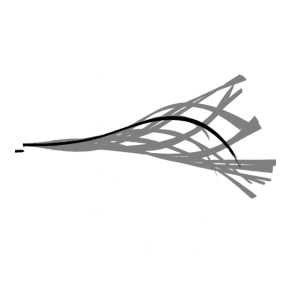
\includegraphics[width=10cm,trim=0 2cm 0cm 1.7cm,clip]{2D_flag_snapshots}};
		\node(fig_2d) at(-6,1.1){};
		% 	\fill[pattern=north east lines](fig_2d.west)++(0.3,-1)rectangle++(.3,2);
%		\fill[white](fig_2d.west)++(0,0)rectangle++(1,-1);
		\draw[line width=2mm, fill=white,orange](fig_2d.west)++(.9cm,-1.2cm)node(windtunnel0){}--++(1,0);%node[below,text width=2cm,text =black]{\scriptsize{ wind tunnel wall}};
		\foreach \y in {0.3,0.6,...,2}{
			\draw[->,thick](fig_2d.west)++(1cm,-.75+ \y)--++(1.5,0);  }
		\draw[->,thick](fig_2d.west)++(1,-0.8)--++(1.03,0)node(cp1){};
%		\node[] at([yshift=1.7cm,xshift=1cm]fig_2d.west){$u_\infty$};
		
		\draw[thick](fig_2d.west)++(1,-1.1)..controls ($(cp1)+(0.35,.025)$)..++(1.5,1.3)--++(0,1.);
		
%		\draw[dashed](fig_2d.west)++(-.3,-.7)--++(1.3,0);
%		
%		\draw[-latex](windtunnel0)++(0,-.4)--++(0,.5);
%		\draw[-latex](windtunnel0)++(0,1.1)--++(0,-.5);
%		\node at([yshift=.3cm,xshift=-.3cm]windtunnel0){\small{$\delta\equiv\theta_0$}};
	\end{tikzpicture}
\end{document}